\section{Introduction}
The WLCG strategy paper \cite{wlcg} set out the path towards computing for the HL-LHC era, building up from the input provided by the HSF \cite{hsf} Community White Paper \cite{cwp}.
The estimates for the data volumes and computing show a major step up from the current needs and a program of work was established from the WLCG point of view to address this future challenge. One of the charges is addressed by the DOMA access Working Group to evaluate future data access scenarios.\\
The working group collected information from experiments future plans about analysis data formats, is following-up the work pioneered by the cost model working group to understand file placement and file usage statistics and is investigating data caches infrastructures and promoting the deployment of caching models leveraging data access from a consolidated storage infrastructure labeled as datalake (Fig. ~\ref{datalake-sketch-horizontal}).

\begin{figure}
  \centering
  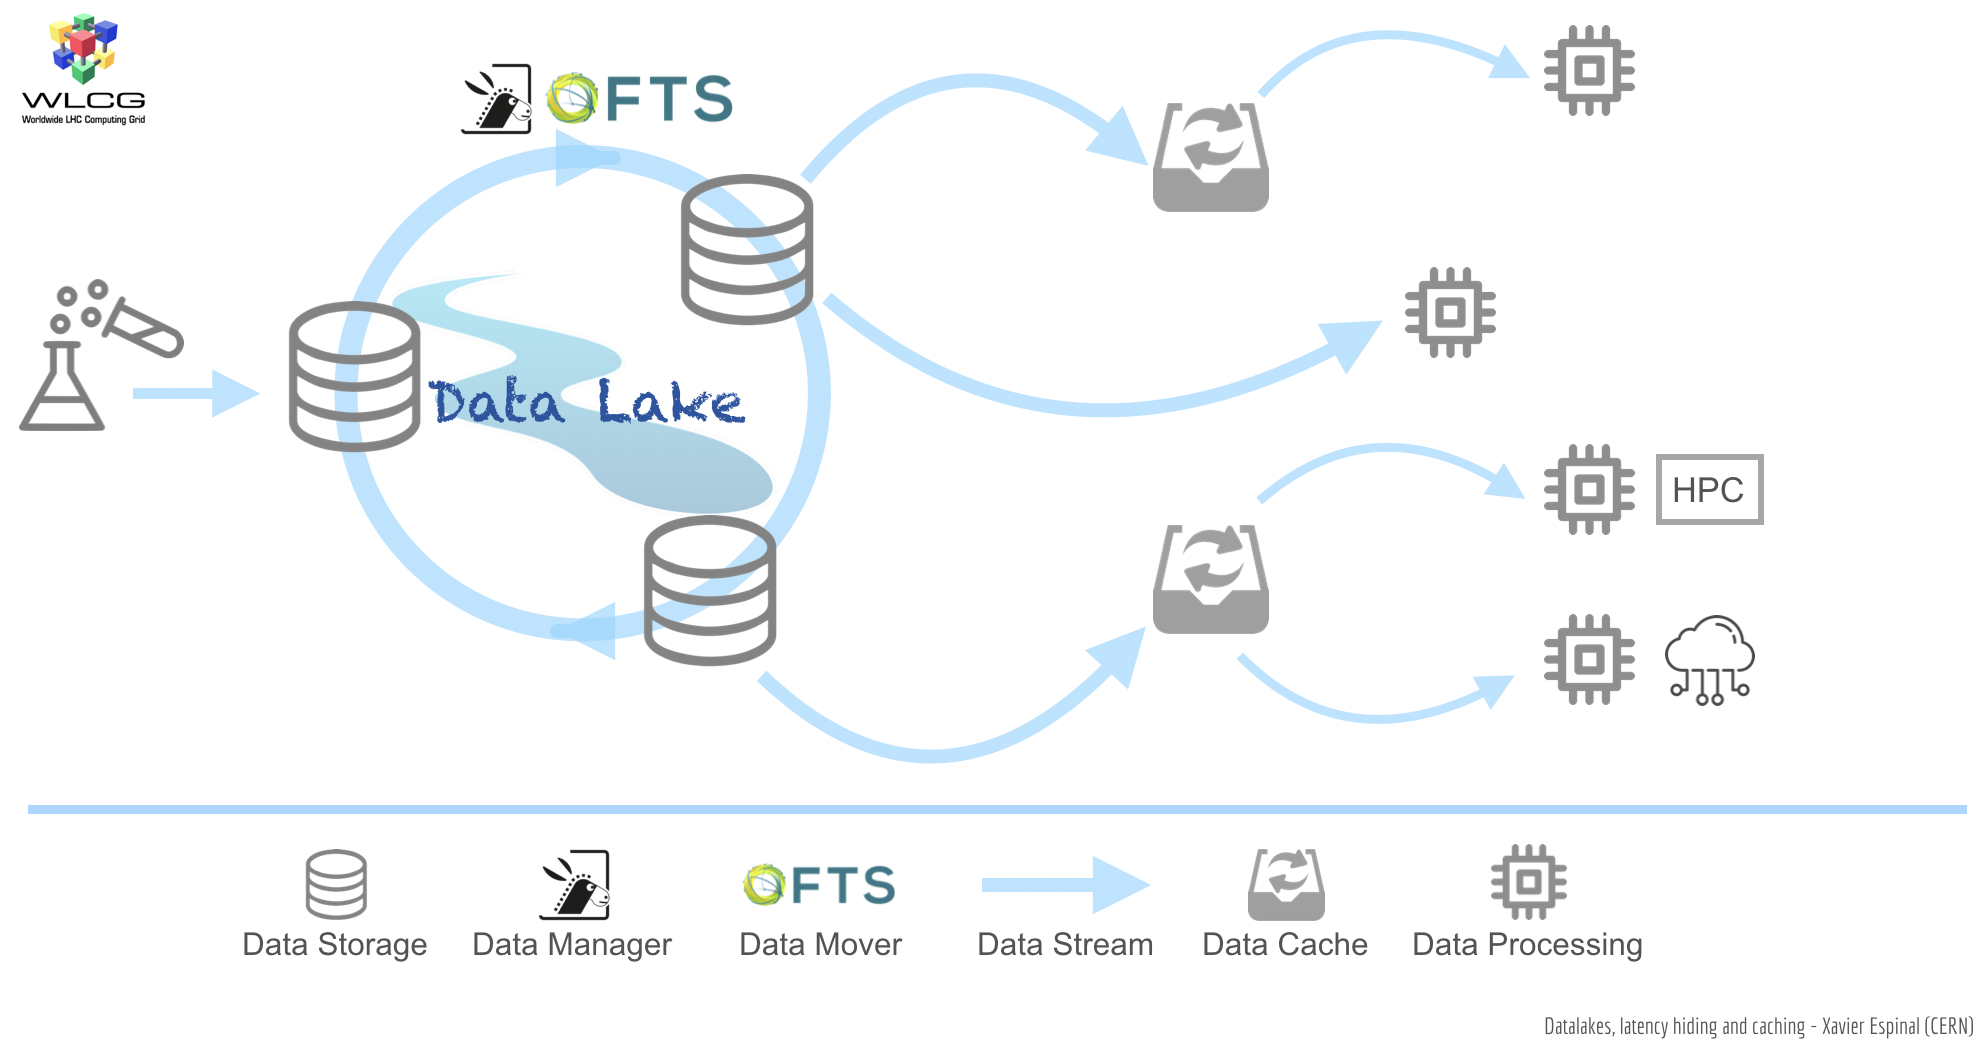
\includegraphics[height=6cm]{Datalake-sketch-horizontal.png}
  \caption{{\em} Conceptual sketch of the datalake idea}
  \label{datalake-sketch-horizontal}
\end{figure}



